% fig_1_Y_inverted_triangle -- TikZ source of thesis Figure 1 (fig:inverted_triangle).
% Every label and number is taken from the text of thesis Chapter 1.
% Sizes (KTU thesis guide, section 5.1: figure text >= 10 pt): body text 10.1 pt, tier headings 11 pt bold; the
% tiers are proportioned (wide, tall, gentle common slope) so that the figure is ~15.4 cm wide and is included at
% \includegraphics[width=\textwidth] (scale ~1.0).
\documentclass[border=1pt]{standalone}
\usepackage[T1]{fontenc}
\usepackage{newtxtext,newtxmath}
\usepackage{amsmath}
\usepackage{tikz}

% ---- sizes: printed >= 10 pt at scale ~1 (10.1 TeX pt = 10.06 bp) ----
\newcommand{\bodysize}{\fontsize{10.1}{12.4}\selectfont}
\newcommand{\headsize}{\fontsize{11}{13.4}\selectfont\bfseries}
\DeclareMathSizes{10.1}{10.1}{7.07}{5.05}
\DeclareMathSizes{11}{11}{7.7}{5.5}

% Print-safe fills: one hue, luminance ~93% / 87% / 80% (stronger towards the focus), black text.
\definecolor{tierA}{RGB}{234,240,247}
\definecolor{tierB}{RGB}{214,226,240}
\definecolor{tierC}{RGB}{192,210,232}
\definecolor{edge}{RGB}{55,75,105}

\newcommand{\Wd}{15.30} % drawing width (cm); + border and line width = ~15.4 cm
\newcommand{\Sl}{0.26}  % side inset per cm of depth (common slope of all tiers)
% \tier{depth of top edge}{depth of bottom edge}{fill colour}
\newcommand{\tier}[3]{%
  \filldraw[fill=#3, draw=edge, line width=0.6pt, line join=round]
    ({\Sl*#1}, {-#1}) -- ({\Wd-\Sl*#1}, {-#1}) -- ({\Wd-\Sl*#2}, {-#2}) -- ({\Sl*#2}, {-#2}) -- cycle;}

\begin{document}
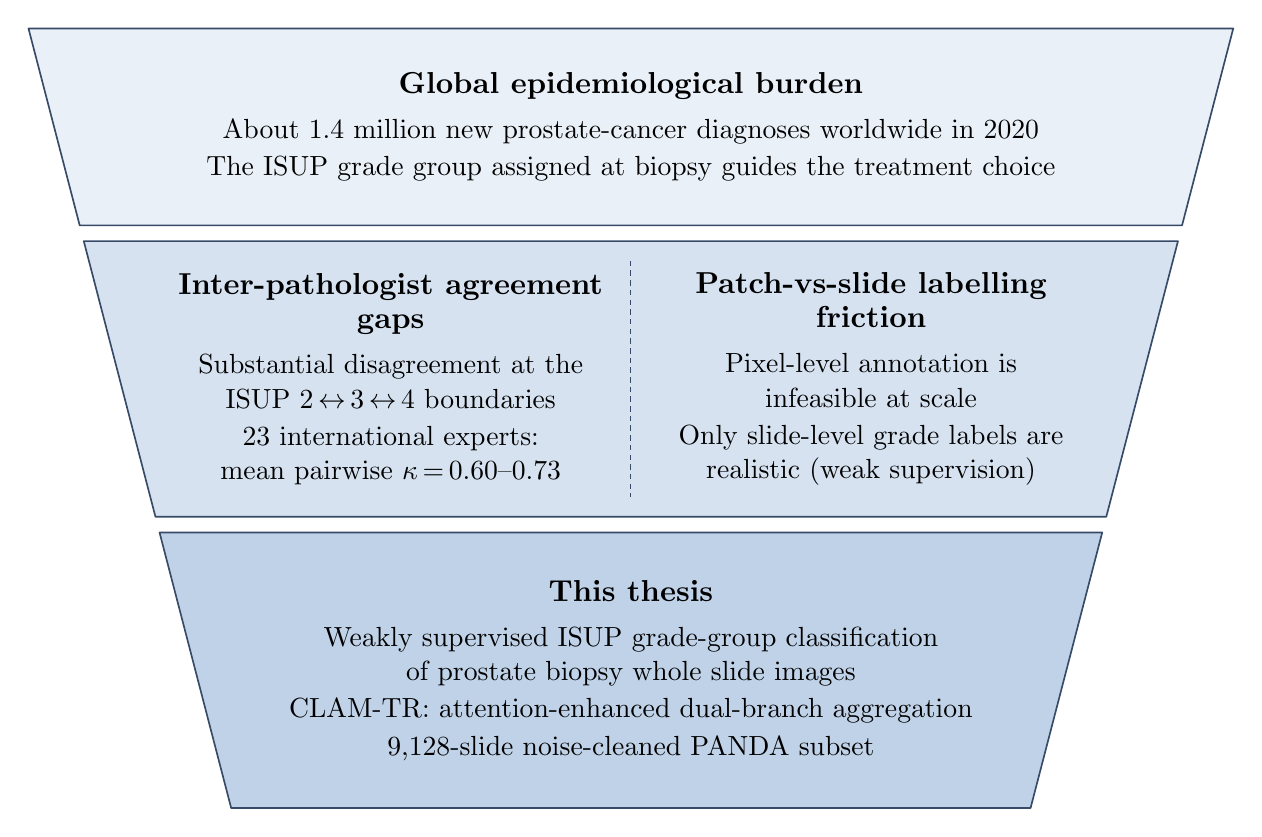
\begin{tikzpicture}[x=1cm, y=1cm,
    body/.style={font=\bodysize, align=flush center, inner sep=0pt,
                 execute at begin node={\hyphenpenalty=10000\exhyphenpenalty=10000}}]

  % ---- three tiers of the inverted triangle ----
  \tier{0}{2.5}{tierA}
  \tier{2.7}{6.2}{tierB}
  \tier{6.4}{9.9}{tierC}

  % ---- tier 1: broad problem ----
  \node[body, text width=12.4cm] at (7.65,-1.25) {%
    {\headsize Global epidemiological burden}\\[4pt]
    About 1.4 million new prostate-cancer diagnoses worldwide in 2020\\[1pt]
    The ISUP grade group assigned at biopsy guides the treatment choice};

  % ---- tier 2: specific gap (two halves) ----
  \draw[edge, line width=0.4pt, dash pattern=on 2pt off 1.5pt] (7.65,-2.95) -- (7.65,-5.95);
  \node[body, text width=5.9cm] at (4.60,-4.45) {%
    {\headsize Inter-pathologist agreement gaps}\\[4pt]
    Substantial disagreement at the\\ ISUP 2\,$\leftrightarrow$\,3\,$\leftrightarrow$\,4 boundaries\\[1pt]
    23 international experts:\\ mean pairwise $\kappa$\,=\,0.60--0.73};
  \node[body, text width=5.9cm] at (10.70,-4.45) {%
    {\headsize Patch-vs-slide labelling friction}\\[4pt]
    Pixel-level annotation is\\ infeasible at scale\\[1pt]
    Only slide-level grade labels are\\ realistic (weak supervision)};

  % ---- tier 3: this thesis ----
  \node[body, text width=8.8cm] at (7.65,-8.15) {%
    {\headsize This thesis}\\[4pt]
    Weakly supervised ISUP grade-group classification\\ of prostate biopsy whole slide images\\[1pt]
    CLAM-TR: attention-enhanced dual-branch aggregation\\[1pt]
    9,128-slide noise-cleaned PANDA subset};
\end{tikzpicture}
\end{document}
